\documentclass[letterpaper, 10 pt]{report}

% For handling graphics
\usepackage{graphicx}
% For colors
\usepackage{color}
% For hyperlink
\PassOptionsToPackage{hyphens}{url}
\usepackage{hyperref}
\hypersetup{
    colorlinks,
    linktoc=all,
    citecolor=black,
    filecolor=black,
    linkcolor=black,
    urlcolor=blue
}
% For mathematics
\usepackage{mathtools}
\usepackage[margin=1.0in]{geometry}
\usepackage{listings}

% -------------------------------------------------------------------------------------
% TITLE PAGE
% -------------------------------------------------------------------------------------
\begin{document}
\begin{titlepage}
\center
% Headings
\textsc{\LARGE PVLabs}\\[1.5cm]

% Title
\rule{\linewidth}{0.5mm}\\[0.4cm]
{\huge \bfseries PhantomX Reactor Arm Notebook}\\[0.4cm]
\rule{\linewidth}{0.5mm}\\[1.5cm]
% Author
\textsc{\normalsize Peter Vieira}\\[1.5cm]
% Image
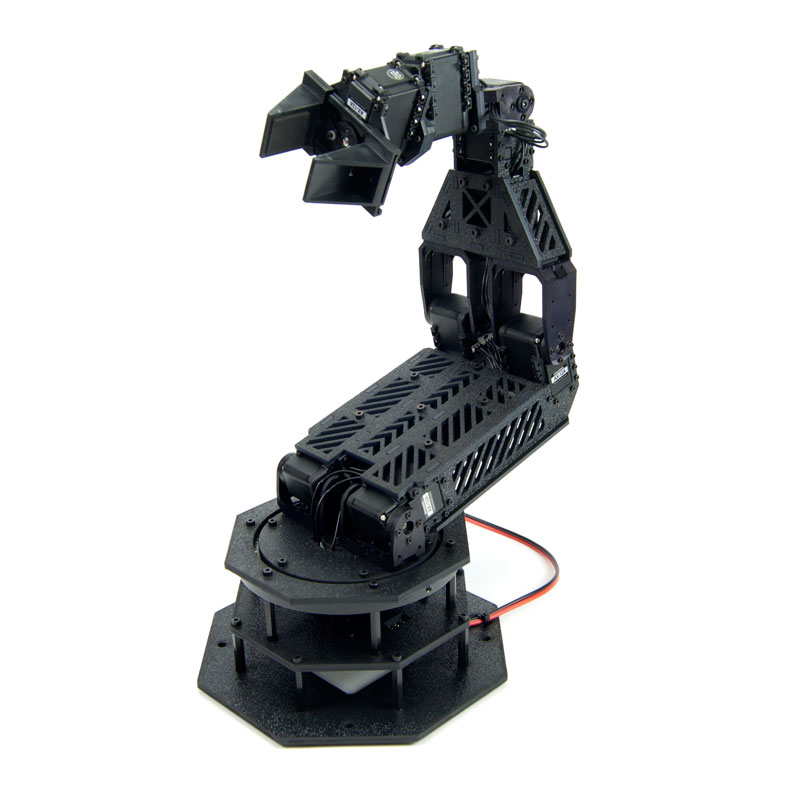
\includegraphics[width=10.0cm]{resources/phantomx-reactor}
% Fill rest of page with whitespace
\vfill
\end{titlepage}

% -------------------------------------------------------------------------------------
% JOURNAL ENTRIES
% -------------------------------------------------------------------------------------


\section*{May 12, 2014}
\subsection*{Communicating with the arm}
\begin{itemize}
  \item XBee wifi module
    \begin{itemize}
      \item Buy the Wifi Trace or PCB version. \url{https://www.sparkfun.com/products/11215}. \$22.95.
      \item Requires USB-to-XBee adapter to program or communicate from a computer
      \item One XBee goes directly on the ArbotiX board and the other goes on the adapter that's plugged into the computer.
    \end{itemize}
  \item USB2Dynamixel Adapter
    \begin{itemize}
      \item \url{http://www.trossenrobotics.com/robotis-bioloid-usb2dynamixel.aspx} \$49.99.
      \item Communicate between computer and Dynamixel motors. So the most logical setup would be to buy a BeagleBone Black and put it on the arm base and communicate with it using a client computer. The USB2Dynamixel adapter to connect to the BeagleBone Black or PandaBoard.
    \end{itemize}
\end{itemize}

% ---------------------

\section*{May 11, 2014}
\subsection*{Building the PhantomX Reactor Arm}
During the building of the PhantomX Reactor arm I came across and learned by mistake several things.
\begin{itemize}
  \item Dynamixel servo IDs
    \begin{itemize}
    \item Set the ID of each servo individually using the dynamanager software before starting to build the robot arm. \url{http://learn.trossenrobotics.com/arbotix/arbotix-getting-started/1-setting-dynamixel-ids-with-the-dynamanager.html#&panel1-1}. I was not able to connect to the servos until I fixed an issue with the RXTXcomm.jar java file.
    \end{itemize}
  \item Accessing the USB port on Linux, Ubuntu 12.04
    \begin{itemize}
      \item The "Serial Port" menu inside the "Tools" menu in the Arduino IDE was greyed out. The problem occurs because of conflicting .jar files. Locate all "RXTXcomm.jar" files and figure out which one is the problem and remove it. For me it was a MATLAB version of the file.
      \item sudo updatedb (update the database)
      \item locate RXTXcomm.jar (locate the file) \newline
      /usr/share/arduino/lib/RXTXcomm.jar \newline
      /usr/share/java/RXTXcomm.jar
      \item I renamed the first one and restarted and everything work fine. I was able to see \textbf{/dev/ttyUSB0}
    \end{itemize}
  \item Connection error
    \begin{itemize}
      \item Before my computer could actually connect to the Arbotix I got the following error when I tried to upload test code: \textbf{"avrdude : stk500\_getsync():not in sync: resp=0x00"} \newline
      This error means the computer can't connect to the board. The fix was to hit the "reset" button on the Arbotix board and power cycle. After that I was able to upload just fine.
    \end{itemize}
  \item Parts Screw-ups
    \begin{itemize}
      \item One standoff was broken
      \item One screw head was melted and unusable
      \item The M2-14 screws were not grade 8 like all the other ones.
    \end{itemize}
  \item Running Arduino Test Code from Sketchbook
    \begin{itemize}
      \item The demo ran fine except that at the beginning the base servo shot to the middle position super fast and terrifyingly. And everytime I powered the arm on, it ran that same test program, so make sure it's in a safe location. The middle position of the servo (the ideal zero position) is located in between 0 and the limit (usually around 300 degrees).
    \end{itemize}
\end{itemize}


% -------------------------------------------------------------------------------------
% REFERENCES
% -------------------------------------------------------------------------------------
%\bibliography{}

% -------------------------------------------------------------------------------------
% END DOCUMENT
% -------------------------------------------------------------------------------------
\end{document}
